\section{Results}

% ------------------------------------------------------------------------------
% src: juliet_full/data/build/probes_layer3.json (eval split, macro-F1; BoW AUROC) via \res{df-x}{probe_*};
%   Clang SA from the registry runs (\res{clang_sa-<layer>}, \res{df-clang_sa}); G2B cue (ALLOCA / new):
%   juliet_full/lane_reports/2026-11-23_data_stage3.md:52
\begin{frame}{DeadFree removes the label shortcuts; one cue is left in G2B goods}
  \slidecite{\bib{clangsa}}
  \centering
  \renewcommand{\arraystretch}{1.15}
  \begin{tabular}{@{}lccc@{}}
    \toprule
    Shortcut probe (macro-F1) & Original & Debiased & DeadFree \\
    \midrule
    grep: no \code{free}/\code{delete} $\Rightarrow$ leak & \alert{\res{df-x}{probe_grep_v0_original}} & \res{df-x}{probe_grep_v0_layer1} & \res{df-x}{probe_grep_v0_layer3} \\
    \code{static void} $\Rightarrow$ good & \alert{\res{df-x}{probe_static_void_original}} & \res{df-x}{probe_static_void_layer1} & \res{df-x}{probe_static_void_layer3} \\
    bag-of-words logistic regression & \alert{\res{df-x}{probe_bow_lr_original}} & \res{df-x}{probe_bow_lr_layer1} & \res{df-x}{probe_bow_lr_layer3} \\
    \quad AUROC, B2G goods & \res{df-x}{probe_bow_auroc_B2G_original} & \res{df-x}{probe_bow_auroc_B2G_layer1} & \res{df-x}{probe_bow_auroc_B2G_layer3} \\
    \quad AUROC, G2B goods & \res{df-x}{probe_bow_auroc_G2B_original} & \res{df-x}{probe_bow_auroc_G2B_layer1} & \textcolor{OIvermil}{\res{df-x}{probe_bow_auroc_G2B_layer3}} \\
    \midrule
    \textcolor{NeutDraw}{Clang SA (reference)} & \textcolor{NeutDraw}{\res{clang_sa-original}{macro}} & \textcolor{NeutDraw}{\res{clang_sa-layer1}{macro}} & \textcolor{NeutDraw}{\res{df-clang_sa}{macro}} \\
    \bottomrule
  \end{tabular}
  \vspace{8pt}
  \begin{itemize}
    \item Residual: G2B goods still use \code{ALLOCA} or \code{new} instead of \code{malloc}
    \item \textbf{From here on, every model is compared on DeadFree only}
  \end{itemize}
\end{frame}

% ------------------------------------------------------------------------------
\begin{frame}{Two cloud services, three local models, one fine-tuned model}
  \slidecite{\bib{deepseekdocs}; \bib{deepseek2026v4}; \bib{typesafe2026jev}; \bib{qwen35card}; \bib{zhu2026interndecision}; \bib{nie2025vulnllmr}; \bib{hu2022lora}; \bib{clangsa}; \bib{inferpulse}; \bib{codeqldocs}; \bib{lsan}}
  \centering
  \footnotesize
  \renewcommand{\arraystretch}{1.05}
  \begin{tabular}{@{}llll@{}}
    \toprule
    Model & Where & Kind & Role \\
    \midrule
    DeepSeek V4.1 Flash & cloud API & generative & cloud reference (L1--L4) \\
    Jev (TypeSafe) & cloud API & decision & cloud reference (L1--L3, L4-D) \\
    \midrule
    Qwen3.5-4B & RTX 3090 & generative & LLM baseline \\
    Qwen read-out & RTX 3090 & decision (untuned) & starting point of our LoRA \\
    Intern-Decision-4B & RTX 3090 & decision & untuned decision baseline \\
    VulnLLM-R-7B & RTX 3090 & generative & vulnerability-tuned, published \\
    \textbf{ours}: Qwen3.5-4B + LoRA & RTX 3090 & decision & fine-tuned per strategy \\
    \midrule
    \textcolor{NeutDraw}{Clang SA, Infer, CodeQL, \dots} & \textcolor{NeutDraw}{CPU} & \textcolor{NeutDraw}{static} & \textcolor{NeutDraw}{tool reference} \\
    \textcolor{NeutDraw}{ASan/LSan, coverage + trace} & \textcolor{NeutDraw}{CPU} & \textcolor{NeutDraw}{dynamic} & \textcolor{NeutDraw}{runs the code} \\
    \bottomrule
  \end{tabular}
  \vfill
  {\scriptsize \textbf{Qwen read-out} = untuned Qwen3.5-4B used as a decision model: same yes/no question, read P(Yes) vs P(No) instead of letting it write. This is exactly our LoRA's starting point.\par}
\end{frame}

% ------------------------------------------------------------------------------
% src: figures/df_track_generative.tex, figures/df_track_decision.tex <- juliet_full/analysis/deadfree/deadfree_quality.json
%   (methods.json deadfree.tracks; bold = best cell per row, computed); jev_l4d prints "pending" until its row exists.
%   No L2 for read-out / FT: decided PLAN.md:35 (user, 2026-11-24 19:05: FT saw ~1,800 labelled units, L2 prompt 2.4x longer);
%   training units per fold 1,712-1,808: PLAN.md:110.
\begin{frame}{Two tracks $\times$ four strategies (DeadFree)}
  \slidecite{\bib{deepseekdocs}; \bib{typesafe2026jev}; \bib{qwen35card}; \bib{zhu2026interndecision}; \bib{hu2022lora}}
  \begin{columns}[T]
    \begin{column}{0.47\textwidth}
      {\small\textbf{Generative}: writes text, we parse it}\\[1pt]
      {\footnotesize\setlength{\tabcolsep}{3.5pt}% generated by figures/make_figures.py from juliet_full/analysis/deadfree/deadfree_quality.json
\begin{tabular}{@{}lcccc@{}}
\toprule
 & L1 & L2 & L3 & L4 \\
\midrule
Qwen3.5-4B & 0.533 & 0.595 & \textbf{0.760} & 0.706 \\
\midrule
DeepSeek (cloud) & 0.863 & 0.873 & 0.875 & \textbf{0.900} \\
\bottomrule
\end{tabular}
}
    \end{column}
    \begin{column}{0.51\textwidth}
      {\small\textbf{Decision}: one pass, read P(Yes) vs P(No)}\\[1pt]
      {\footnotesize\setlength{\tabcolsep}{3.5pt}% generated by figures/make_figures.py from juliet_full/analysis/deadfree/deadfree_quality.json
\begin{tabular}{@{}lcccc@{}}
\toprule
 & L1 & L2 & L3 & L4-D \\
\midrule
Qwen read-out & 0.351 & --$^\dagger$ & 0.334 & \textbf{0.752} \\
Intern-Decision & 0.584 & 0.500 & 0.664 & \textbf{0.799} \\
ours (LoRA) & 0.372 & --$^\dagger$ & 0.639 & \textbf{0.826} \\
\midrule
Jev (cloud) & 0.946 & 0.942 & \textbf{0.949} & 0.907 \\
\bottomrule
\end{tabular}
}
    \end{column}
  \end{columns}
  \footnotesize
  \begin{itemize}
    \item Cloud generative gains from writing facts (DeepSeek L4 \res{df-deepseek_L4}{macro}); the 4B model writes them poorly (L4 \res{df-qwen_L4}{macro} < L3 \res{df-qwen_L3}{macro})
    \item L4-D is the best strategy of every local decision model
    \item Same Qwen weights: \emph{asking} the facts (read-out L4-D \res{df-readout_l4d}{macro}) beats \emph{writing} them (gen.\ L4 \res{df-qwen_L4}{macro})
  \end{itemize}
  \vfill
  {\scriptsize Macro-F1; bold = best per row. Jev L4-D = cloud ceiling of the decision track.\\
  $^\dagger$Not run: FT already saw $\approx$1,800 labelled units; the L2 prompt is 2.4$\times$ longer.\par}
\end{frame}

% ------------------------------------------------------------------------------
% src: figures/df_before_after.pdf <- deadfree_quality.json strategy_x_ft (before: read-out = untuned Qwen3.5-4B weights;
%   after: lora_L1, lora_L3, lora_l4d_opt; marks: Intern-Decision, Qwen gen.); paired delta: deadfree_quality.json
%   paired_deltas; Debiased LoRA L1: registry lora_L1 layer1 (figures/numbers.tex \res{lora_L1-layer1})
\begin{frame}{FT: unit labels stay below the baselines, fact labels beat them}
  \slidecite{\bib{qwen35card}; \bib{hu2022lora}; \bib{zhu2026interndecision}; \bib{efron1979}}
  \centering
  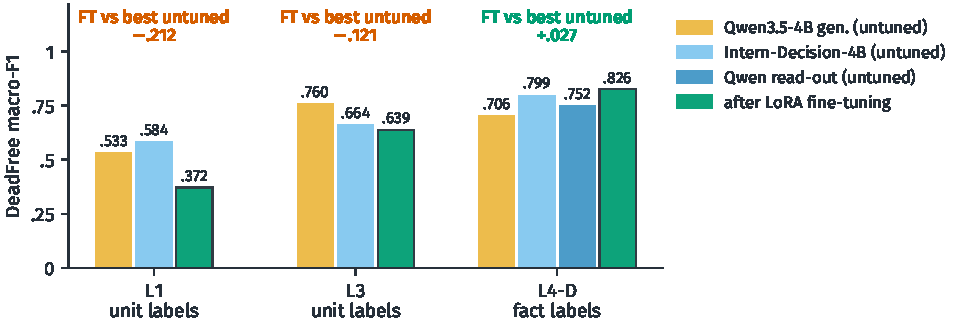
\includegraphics[width=\linewidth,height=0.46\textheight,keepaspectratio]{figures/df_before_after.pdf}\\[0pt]
  \raggedright\footnotesize
  \begin{itemize}
    \item L1/L3 learn \emph{unit labels} $\to$ the shortcut ``a \code{free} means no leak'': FT L1 scores \res{lora_L1-layer1}{macro} on Debiased, \alert{\res{df-lora_L1}{macro}} on DeadFree (leak recall \res{df-lora_L1}{r})
    \item L4-D learns \emph{fact labels} from dynamic analysis $\to$ transfers: \res{df-readout_l4d}{macro} $\to$ \textbf{\res{df-lora_l4d_opt}{macro}};
    vs untuned Intern L4-D \res{df-x}{pd_lora_l4d_opt__intern_l4d} \res{df-x}{pd_lora_l4d_opt__intern_l4d_ci}
  \end{itemize}
  \vfill
  {\scriptsize Same Qwen3.5-4B weights before (read-out) and after (LoRA). Intern-Decision at $\tau=0.5$. $\Delta$ CI: paired family-cluster bootstrap.\par}
\end{frame}

% ------------------------------------------------------------------------------
% src: figures/df_pareto.pdf <- deadfree_quality.json (macro_f1) x latency_deadfree.csv (median_s, log axis);
%   front over model-based methods; static tools grey; dynamic analysis dashed reference
\begin{frame}{FT L4-D is the most accurate local model, still below the cloud}
  \slidecite{\bib{deepseekdocs}; \bib{typesafe2026jev}; \bib{zhu2026interndecision}; \bib{nie2025vulnllmr}; \bib{clangsa}; \bib{inferpulse}; \bib{codeqldocs}; \bib{cppcheck}; \bib{serebryany2012asan}}
  \centering
  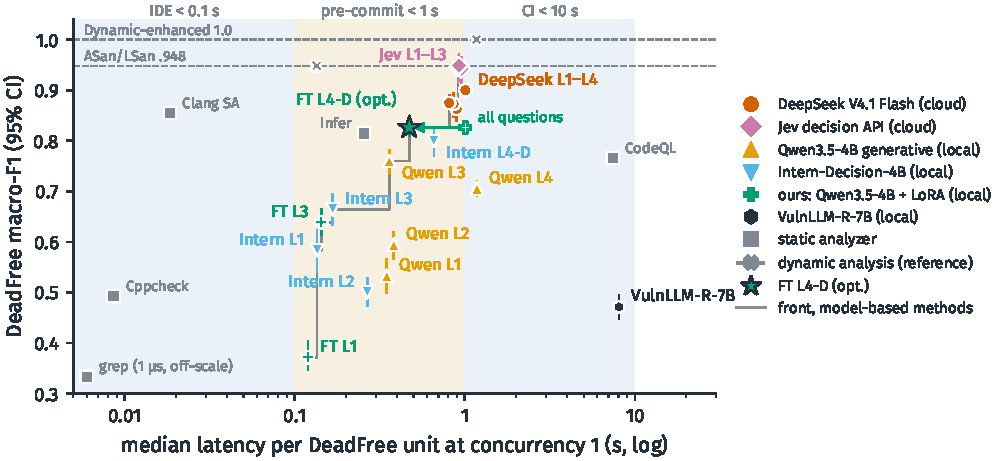
\includegraphics[width=\linewidth,height=0.70\textheight,keepaspectratio]{figures/df_pareto.pdf}
  \vfill
  {\scriptsize x: median latency per DeadFree unit, concurrency 1 (log); y: macro-F1 with 95\,\% CI.
  Shape = track, colour = cloud / local; grey: static tools; dashed: dynamic analysis (reference).\par}
\end{frame}

% ------------------------------------------------------------------------------
% src: deadfree_quality.json lora_l4d_opt / intern_l4d / clang_sa / jev_L3 / jev_l4d (pending until JEV_L4D_READY): delta_vs_ds_l1(_ci), gap_closed_ds_l1(_ci), delta_vs_ds_l4(_ci),
%   gap_closed_ds_l4(_ci); family-cluster bootstrap. Criterion pre-registered PLAN.md:224-226 (2026-11-23 22:30 PST,
%   before L4-D ran): near if macro-F1 point estimate >= reference - 0.02; reported as not met PLAN.md:34.
\begin{frame}{L4-D closes \res{df-intern_l4d}{gap1} of the gap untuned, \res{df-lora_l4d_opt}{gap1} fine-tuned; not near-cloud}
  \slidecite{\bib{deepseekdocs}; \bib{typesafe2026jev}; \bib{efron1979}}
  \centering
  \renewcommand{\arraystretch}{1.2}
  {\small
  \begin{tabular}{@{}llcc@{}}
    \toprule
    & vs & $\Delta$ macro-F1 [95\,\% CI] & gap closed \\
    \midrule
    Intern L4-D (untuned) & DeepSeek L1 (\res{df-deepseek_L1}{macro}) & \res{df-intern_l4d}{d1} \res{df-intern_l4d}{d1ci} & \res{df-intern_l4d}{gap1} \\
    \textbf{FT L4-D (opt.)} & DeepSeek L1 (\res{df-deepseek_L1}{macro}) & \res{df-lora_l4d_opt}{d1} \res{df-lora_l4d_opt}{d1ci} & \textbf{\res{df-lora_l4d_opt}{gap1}} \\
    \textbf{FT L4-D (opt.)} & DeepSeek L4 (\res{df-deepseek_L4}{macro}) & \res{df-lora_l4d_opt}{d4} \res{df-lora_l4d_opt}{d4ci} & \res{df-lora_l4d_opt}{gap4} \\
    \bottomrule
  \end{tabular}}\par
  \vspace{8pt}
  \begin{itemize}
    \item Gap measured from untuned Qwen L1 (\res{df-qwen_L1}{macro}) to the cloud model
    \item Criterion: $\geq$ reference $- 0.02$. \alert{Not met}: \res{df-lora_l4d_opt}{d1} vs DeepSeek L1
    \item Median latency: FT L4-D \res{df-lora_l4d_opt}{lat}, Intern L4-D \res{df-intern_l4d}{lat}, DeepSeek L1 \res{df-deepseek_L1}{lat} (FT L4-D \res{df-x}{speedup_ds_l1}$\times$ faster)
    \item Decision-track cloud ceiling: Jev L3 \res{df-jev_L3}{macro}, Jev L4-D \res{df-jev_l4d}{macro}
  \end{itemize}
\end{frame}

% ------------------------------------------------------------------------------
% src: figures/demo.tex <- presentation/demo/recordings/<newest stage_final*.json>; L4-D row from the frozen eval run
%   (juliet_full/l4d_ft/results/lora_l4d_opt/{layer1,layer3}/eval_r1_units.jsonl) until stage_final_v2 exists;
%   exec_all(free at line 20) p_yes 1.8e-07: juliet_full/l4d_ft/results/lora_l4d/layer3/eval_r1.jsonl
%   qid layer3/CWE401_Memory_Leak__strdup_char_01__bad/exec_all/s02
\begin{frame}[fragile]{Live: one dead free fools grep and the old LoRA, not L4-D}
  \slidecite{\bib{clangsa}; \bib{deepseekdocs}; \bib{typesafe2026jev}}
  \begin{columns}[T]
    \begin{column}{0.50\textwidth}
      {\small Bad unit \texttt{strdup\_char\_01}, DeadFree version:\par}
\begin{lstlisting}[style=unit]
static const int sym_61 = 4;
...
data = strdup(myString);
printLine(data);
(*\hlc{if(sym\_61 > 4) \{ free(data); \}}*)
\end{lstlisting}
      {\small The free never runs: still a leak.\par}
    \end{column}
    \begin{column}{0.48\textwidth}
      \textcolor{OIvermil}{\textbf{Flips to ``no leak''}}\\
      {\small \res{x}{demo_flipped}\par}
      \vspace{6pt}
      \textcolor{OIblue}{\textbf{Still ``leak''}}\\
      {\small \res{x}{demo_held}\par}
      \vspace{6pt}
      {\small L4-D: \code{exec\_all(free)} = no $\Rightarrow$ not freed $\Rightarrow$ leak\par}
    \end{column}
  \end{columns}
  \vfill
  {\scriptsize Full table in backup. Recording: \texttt{demo/recordings/\res{x}{demo_file}}; L4-D row: \res{x}{demo_has_l4d}.\par}
\end{frame}
